\subsubsection{Trigger Efficiency Measurements}
 
We used the tag and probe method on \dyll~events to provide an unbiased, high-purity, 
lepton sample with which to measure efficiencies.
This method was used successfully by both Tevatron experiments.

Because of the differing kinematics between the \dyll~events and those on which we apply the measured efficiencies,
we split the efficiency measurements into the barrel and endcap regions.
We picked this division because it covers the largest observed variation in efficiency.

We used a single lepton triggered sample available from the Express Stream, 
from which we selected a subset of di-lepton events.
Ultimately we will repeat this using a double lepton triggered sample from the Prompt Reco,
where we select events using one of our tag and probe triggers which are very tight on one lepton,
but loose on the other.

At least one of the leptons, the {\it tag}, was required to pass the full selection criteria criteria 
whilst the other lepton, the {\it probe}, was required to pass a set of identification criteria leaving 
it unbiassed with respect to the criterion under study. 
By requiring that the tag was able to have passed the single lepton trigger on which the events were acquired, 
we reduced the bias due to the trigger on the probe.
Because the analysis uses the same mass window to reduce the \dyll~contribution, 
the tag and probe sample represents an independent control sample.
The tight criteria imposed on the tag coupled with the invariant mass requirement were sufficient to ensure high purity.

To extract the efficiency of offline selection and single trigger efficiency on a per lepton basis, 
we first construct all possible tag-probe pairs in every event.
Because more than one lepton can meet the tag criteria it is possible to use the same event more than once, to find the efficiency

\begin{eqnarray}
\label{eqn:tagAndProbeEfficiencyEqn}
\varepsilon = \frac{2TT + TP}{2TT + TP + TF}.
\end{eqnarray}

Where the event categories are defined as:

\begin{itemize}
	\item 2TT: Both leptons passed the tight criteria, including the trigger. This means that either lepton could be used as a probe, 
	so such events were counted twice.
	\item TP: The probe passed the selection criterion but did not pass the tight criteria.
	\item TF: The probe failed the selection criterion.
\end{itemize}

For the categories to be mutually exclusive it is important to note that the probe definition, 
and the selection criteria studied are always a subset of the tag criteria.
Classifying events and looping over all possible tag-probe combinations are thus equivalent.

To determine the efficiency of the double lepton triggers, we derive the efficiency of the requirements imposed on each leg separately.
This requires a modification to the tag and probe method described above in some cases.
If the trigger objects are saved by the HLT before the requirement that there be two valid objects then
we can check each leg independently of the other using the usual tag and probe method.
If the trigger objects are saved after the requirement that there are two valid objects, then there is 
a 100\% correlation between the decision we can probe on each lepton.
This means that we must pick exactly one tag candidate for each event a priori, which we do 
randomly. 
If the randomly selected tag candidate meets the tight requirements then we are free to 
probe the other lepton.

\subsubsection{Trigger Efficiency Results}

The tag definition:
\begin{itemize}
	\item  Single trigger blah
	\item Full offline electron/muon selection
\end{itemize}
	
The probe definition (muons / electrons):
\begin{itemize}
	\item  Full offline electron/muon selection
\end{itemize}

  
The per electron efficiency for the seeded leg of the double electron trigger is shown in 
Figure \ref{tab:Ele17Ele8TriggerEfficiencySeededLeg} as a function of $p_{T}$ and $\eta$, 
and summarized in Table \ref{tab:Ele17Ele8TriggerEfficiencySeededLeg}. The efficiency for 
the corresponding unseeded leg is shown in Figure 
\ref{fig:Ele17Ele8TriggerEfficiencyUnseededLeg} and summarized in Table 
\ref{tab:Ele17Ele8TriggerEfficiencyUnseededLeg}. The per electron efficiency for the
single electron trigger is shown in Figure \ref{fig:Ele27Efficiency} and summarized
in Table \ref{tab:Ele27Efficiency}. Finally, to combine these measurements into a final per event
trigger efficiency, one has to fold in the $p_{T}$ and $\eta$ kinematic distributions
of the signal sample.


\begin{table}[!ht]
\begin{center}
\begin{tabular}{|c|c|c|} \hline
              & Barrel ( $|\eta|<1.5$ )  & Endcap ( $|\eta|>1.5$ )  \\ 
\hline
20$<p_{T}<$   & 0.9931 + 0.0012 - 0.0014 & 0.9942 + 0.0019 - 0.0026 \\
\hline
\end{tabular}
\caption{Efficiency for the unseeded leg of the double electron trigger 
separately in bins of $p_{T}$ for the barrel and endcap.
\label{tab:Ele17Ele8TriggerEfficiencySeededLeg}}
\end{center}
\end{table}


\begin{figure}[!ht]
\begin{center}
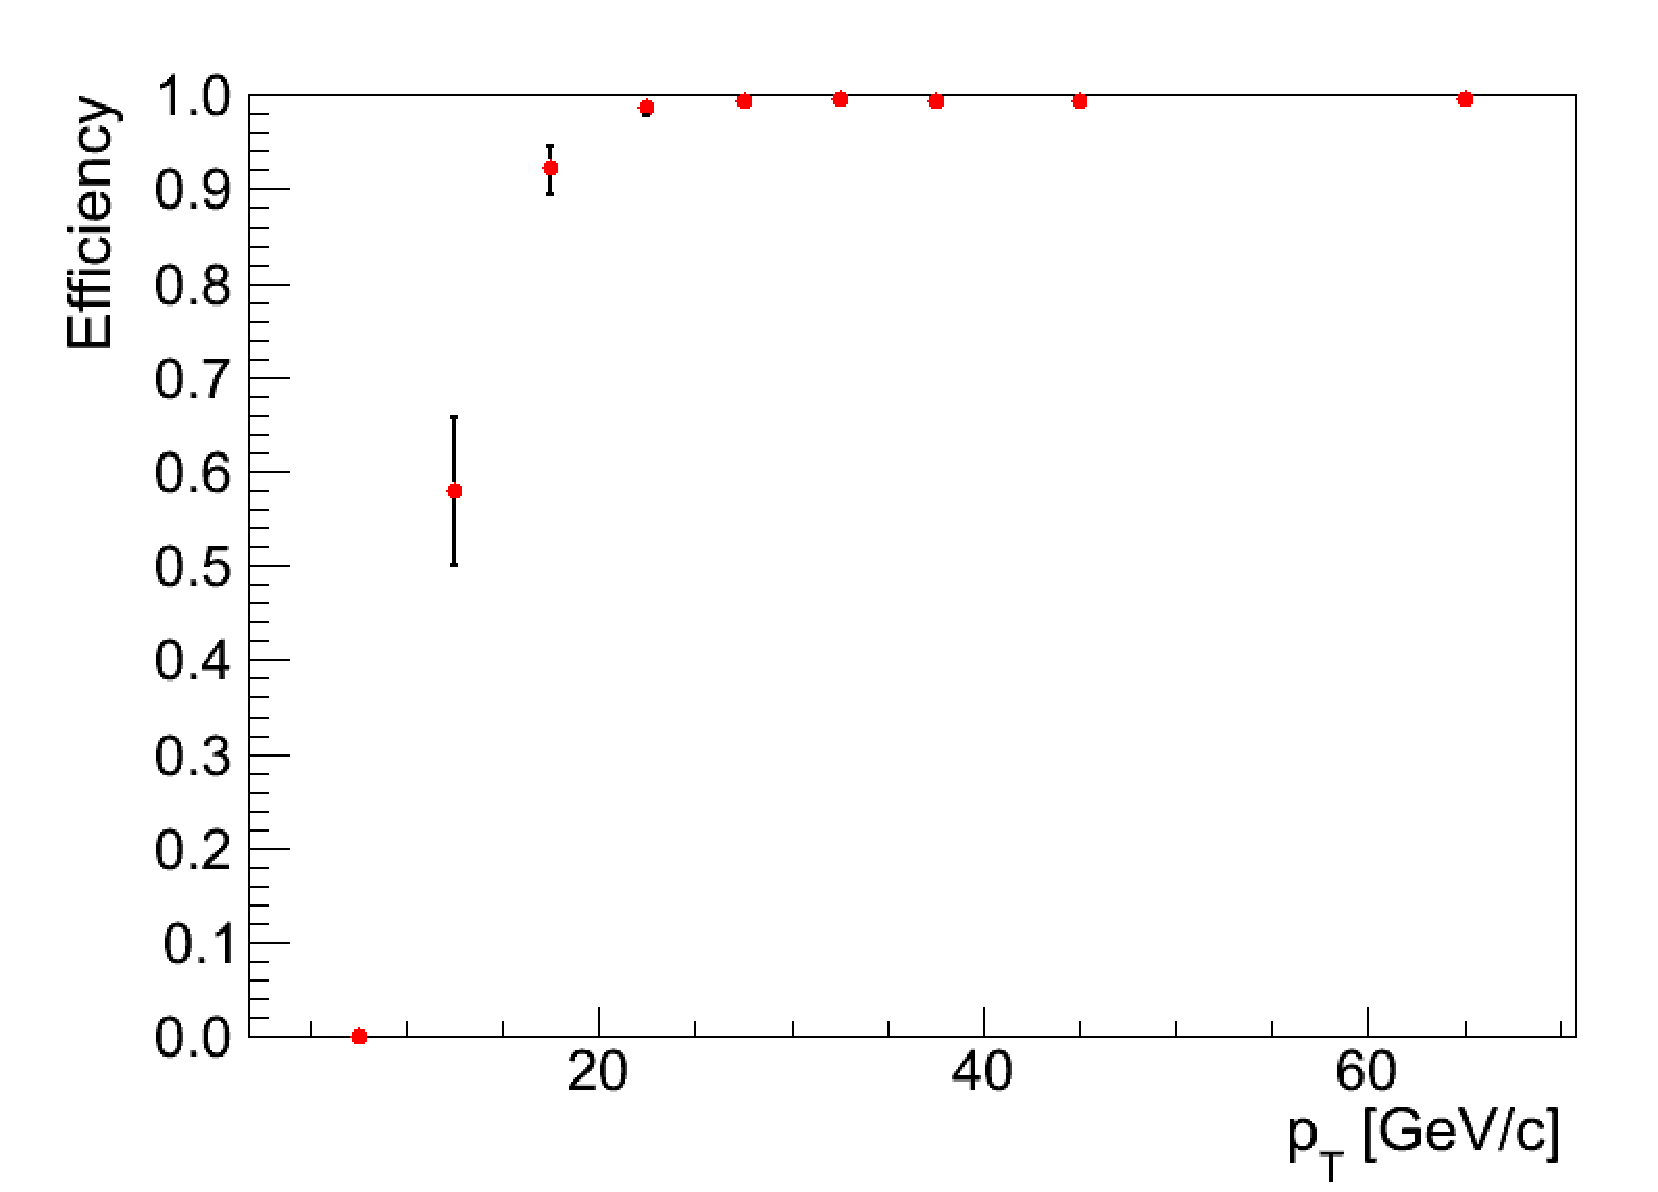
\includegraphics[width=0.48\textwidth]{figures/ElectronTriggerEffVsPt_Ele17Ele8WithL1Seed.pdf}
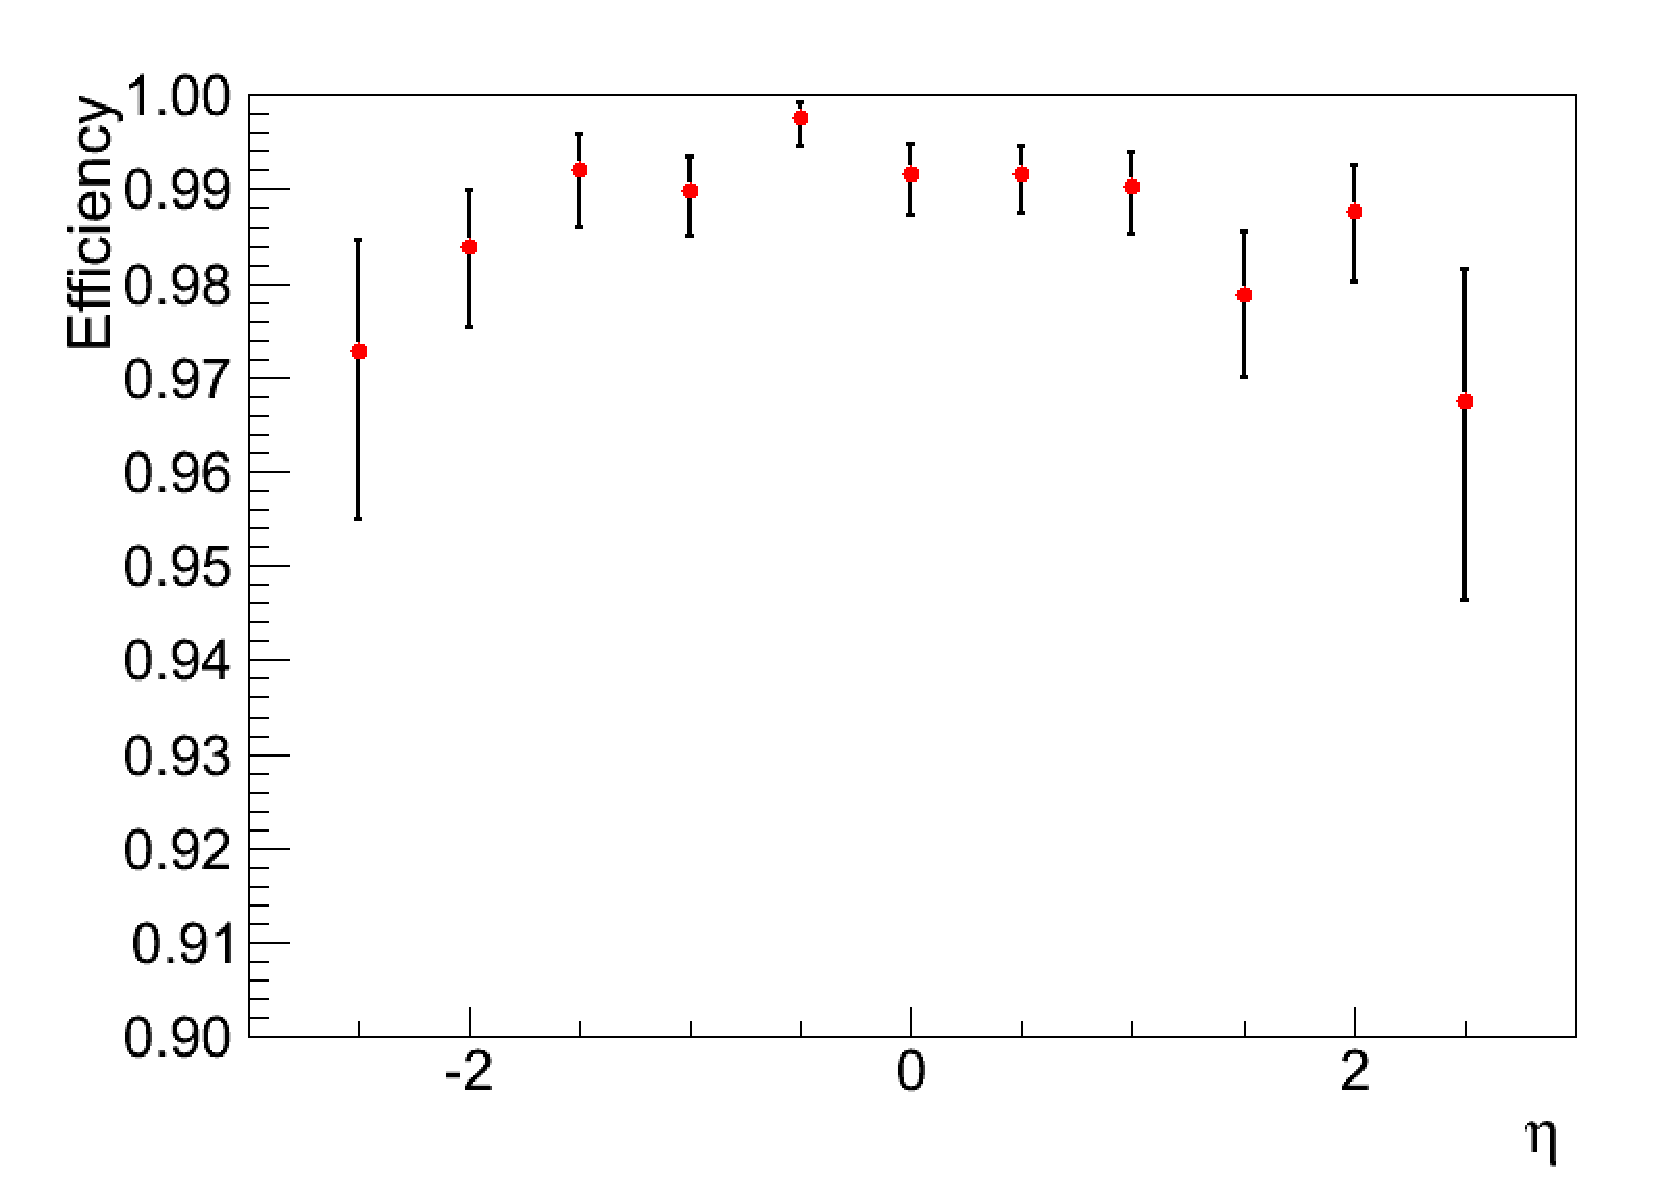
\includegraphics[width=0.48\textwidth]{figures/ElectronTriggerEffVsEta_Ele17Ele8WithL1Seed.pdf}
\end{center}
\caption{Efficiency for the L1 seeded leg of the double electron trigger as a function of $p_{T}$ (a) and $\eta$ (b).}
\label{fig:Ele17Ele8TriggerEfficiencySeededLeg}
\end{figure} 


\begin{table}[!ht]
\begin{center}
\begin{tabular}{|c|c|c|} 
\hline
              & Barrel ( $|\eta|<1.5$ )  & Endcap ( $|\eta|>1.5$ )  \\ 
\hline
10$<p_{T}<$15 & 1.0 + 0.0 - 0.07 & 1.0 + 0.0 - 0.08                 \\
15$<p_{T}<$20 & 1.0 + 0.0 - 0.02 & 0.985 + 0.012 - 0.033            \\
20$<p_{T}<$   & 0.9981 + 0.0006 - 0.0009 & 0.9993 + 0.0005 - 0.0015 \\
\hline
\end{tabular}
\caption{Efficiency for the unseeded leg of the double electron trigger 
separately in bins of $p_{T}$ for the barrel and endcap.
\label{tab:Ele17Ele8TriggerEfficiencyUnseededLeg}}
\end{center}
\end{table}


\begin{figure}[!ht]
\begin{center}
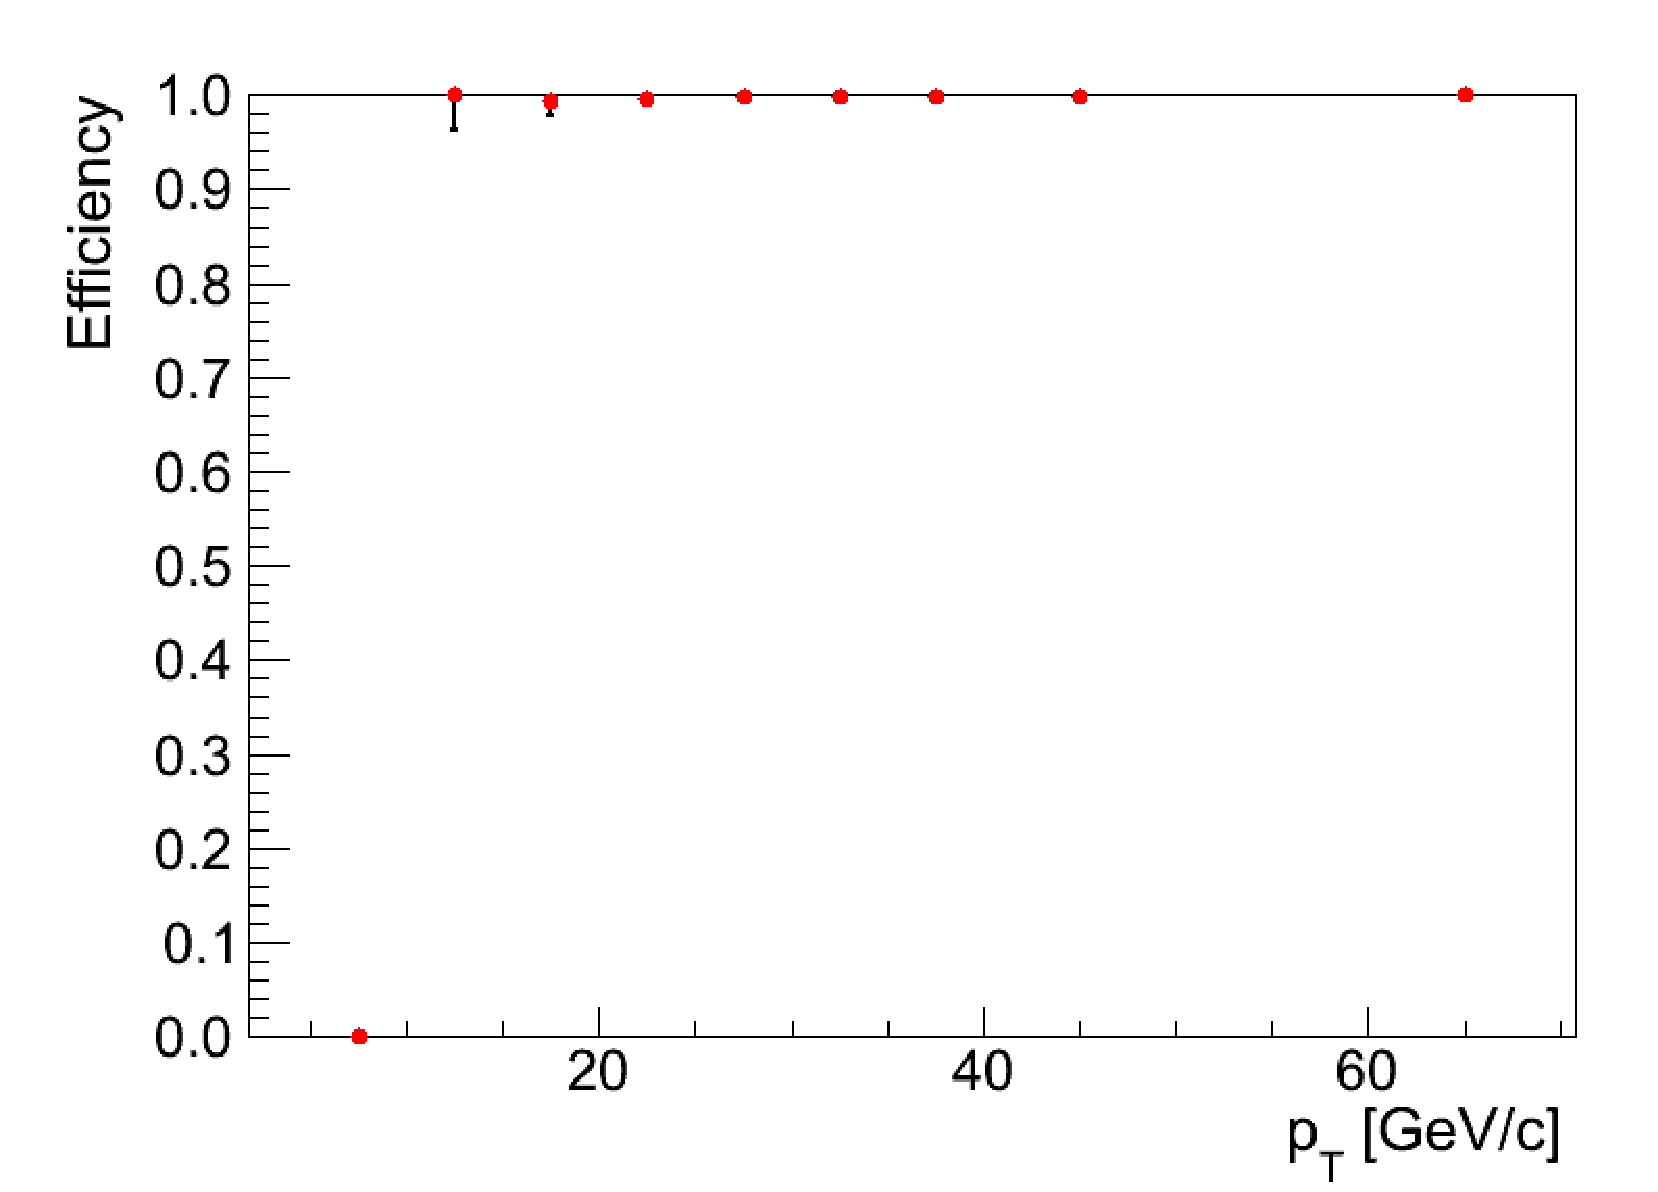
\includegraphics[width=0.48\textwidth]{figures/ElectronTriggerEffVsPt_Ele17Ele8.pdf}
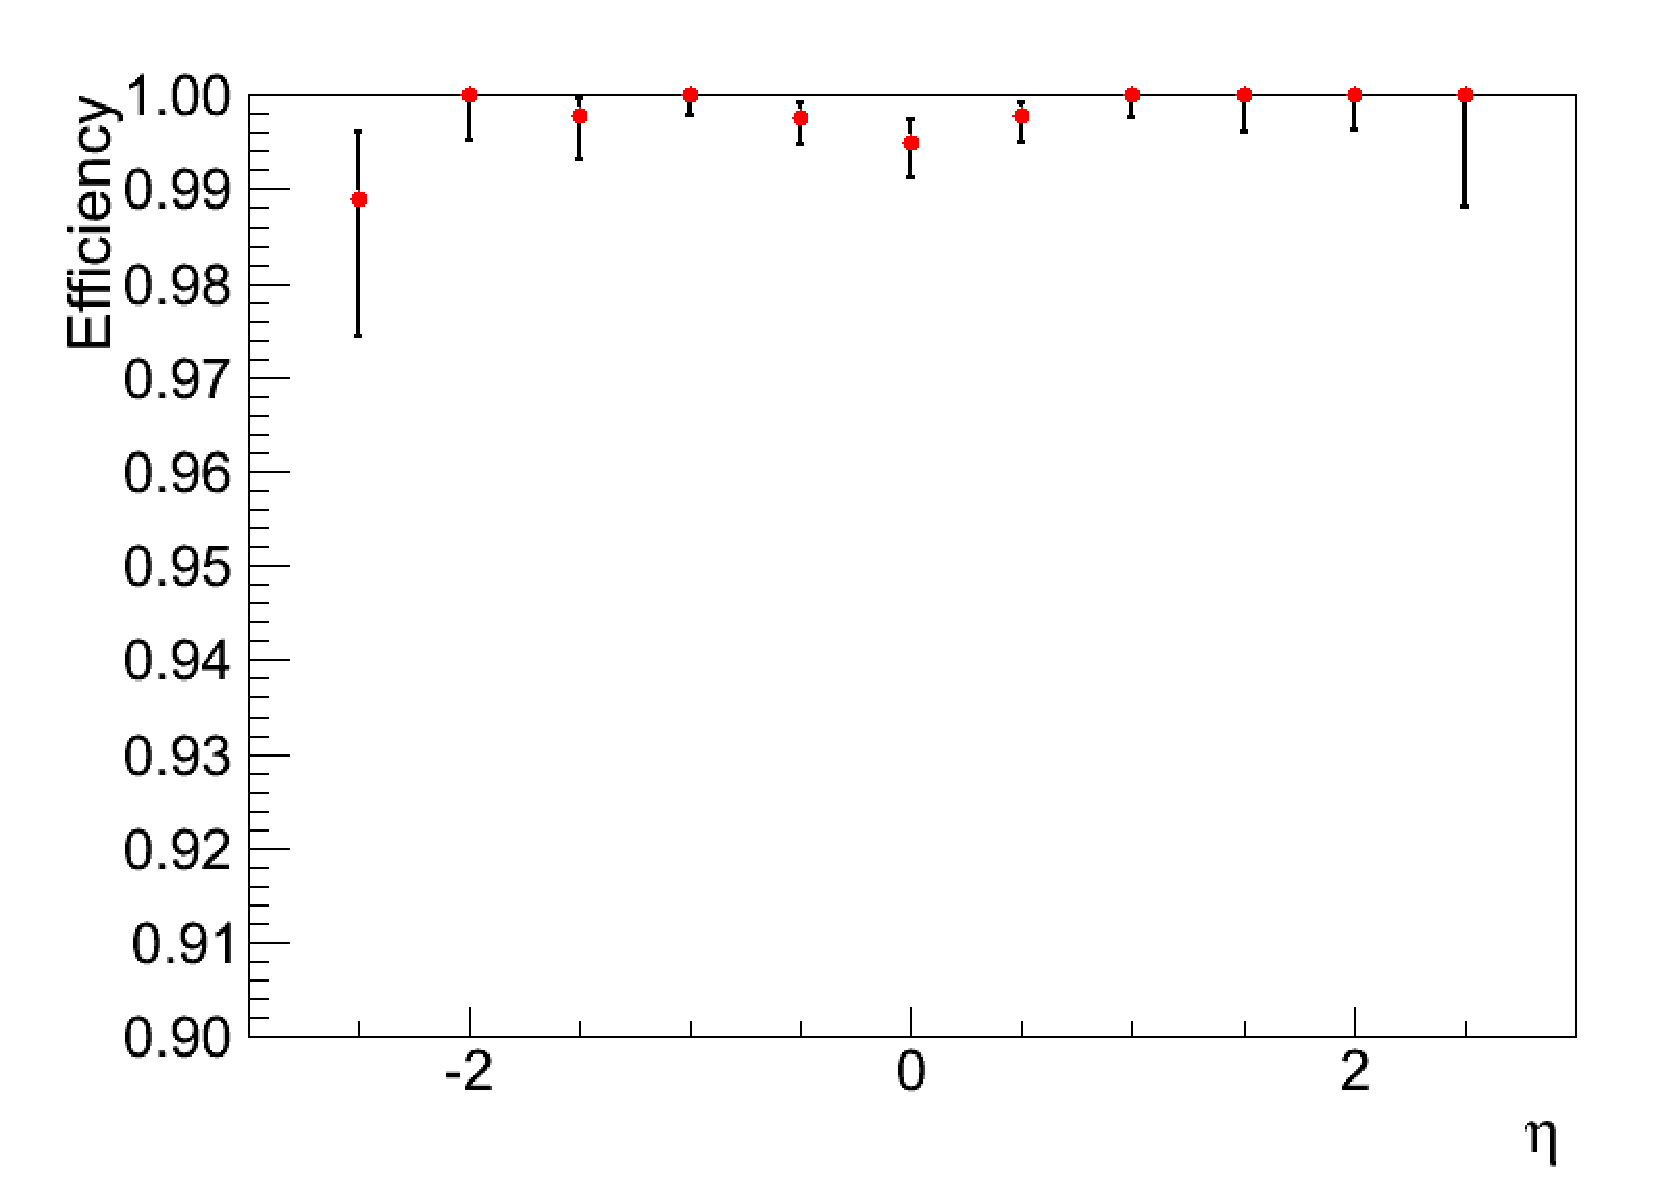
\includegraphics[width=0.48\textwidth]{figures/ElectronTriggerEffVsEta_Ele17Ele8.pdf}
\end{center}
\caption{Efficiency for the unseeded leg of the double electron trigger as a function of $p_{T}$ (a) and $\eta$ (b).}
\label{fig:Ele17Ele8TriggerEfficiencyUnseededLeg}
\end{figure}



\begin{table}[!ht]
\begin{center}
\begin{tabular}{|c|c|c|} \hline
              & Barrel ( $|\eta|<1.5$ )  & Endcap ( $|\eta|>1.5$ )  \\ 
\hline
30$<p_{T}<$   & 0.964 + 0.002 - 0.002 & 0.958 + 0.004 - 0.004 \\
\hline
\end{tabular}
\caption{The single leg efficiency of the single electron trigger 
separately in bins of $p_{T}$ for the barrel and endcap.
\label{tab:Ele27Efficiency}}
\end{center}
\end{table}


\begin{figure}[!ht]
\begin{center}
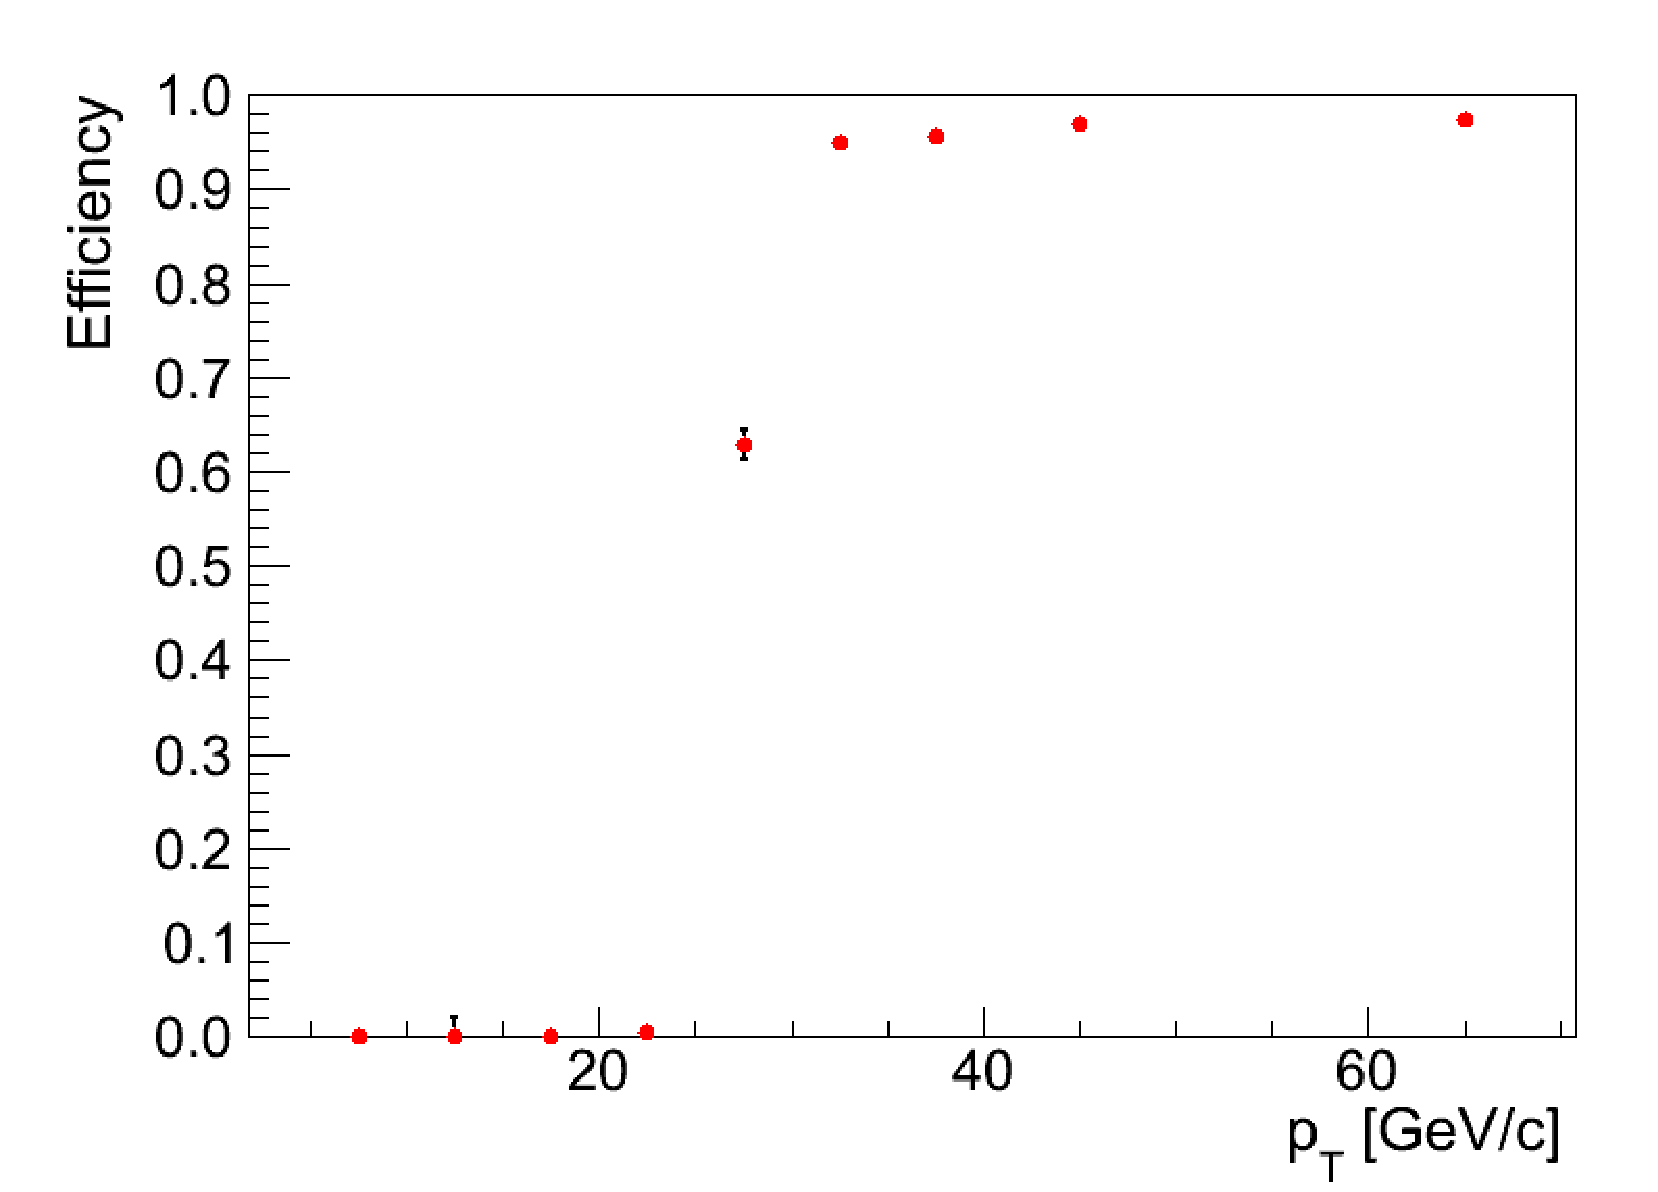
\includegraphics[width=0.48\textwidth]{figures/ElectronTriggerEffVsPt_Ele27Tight.pdf}
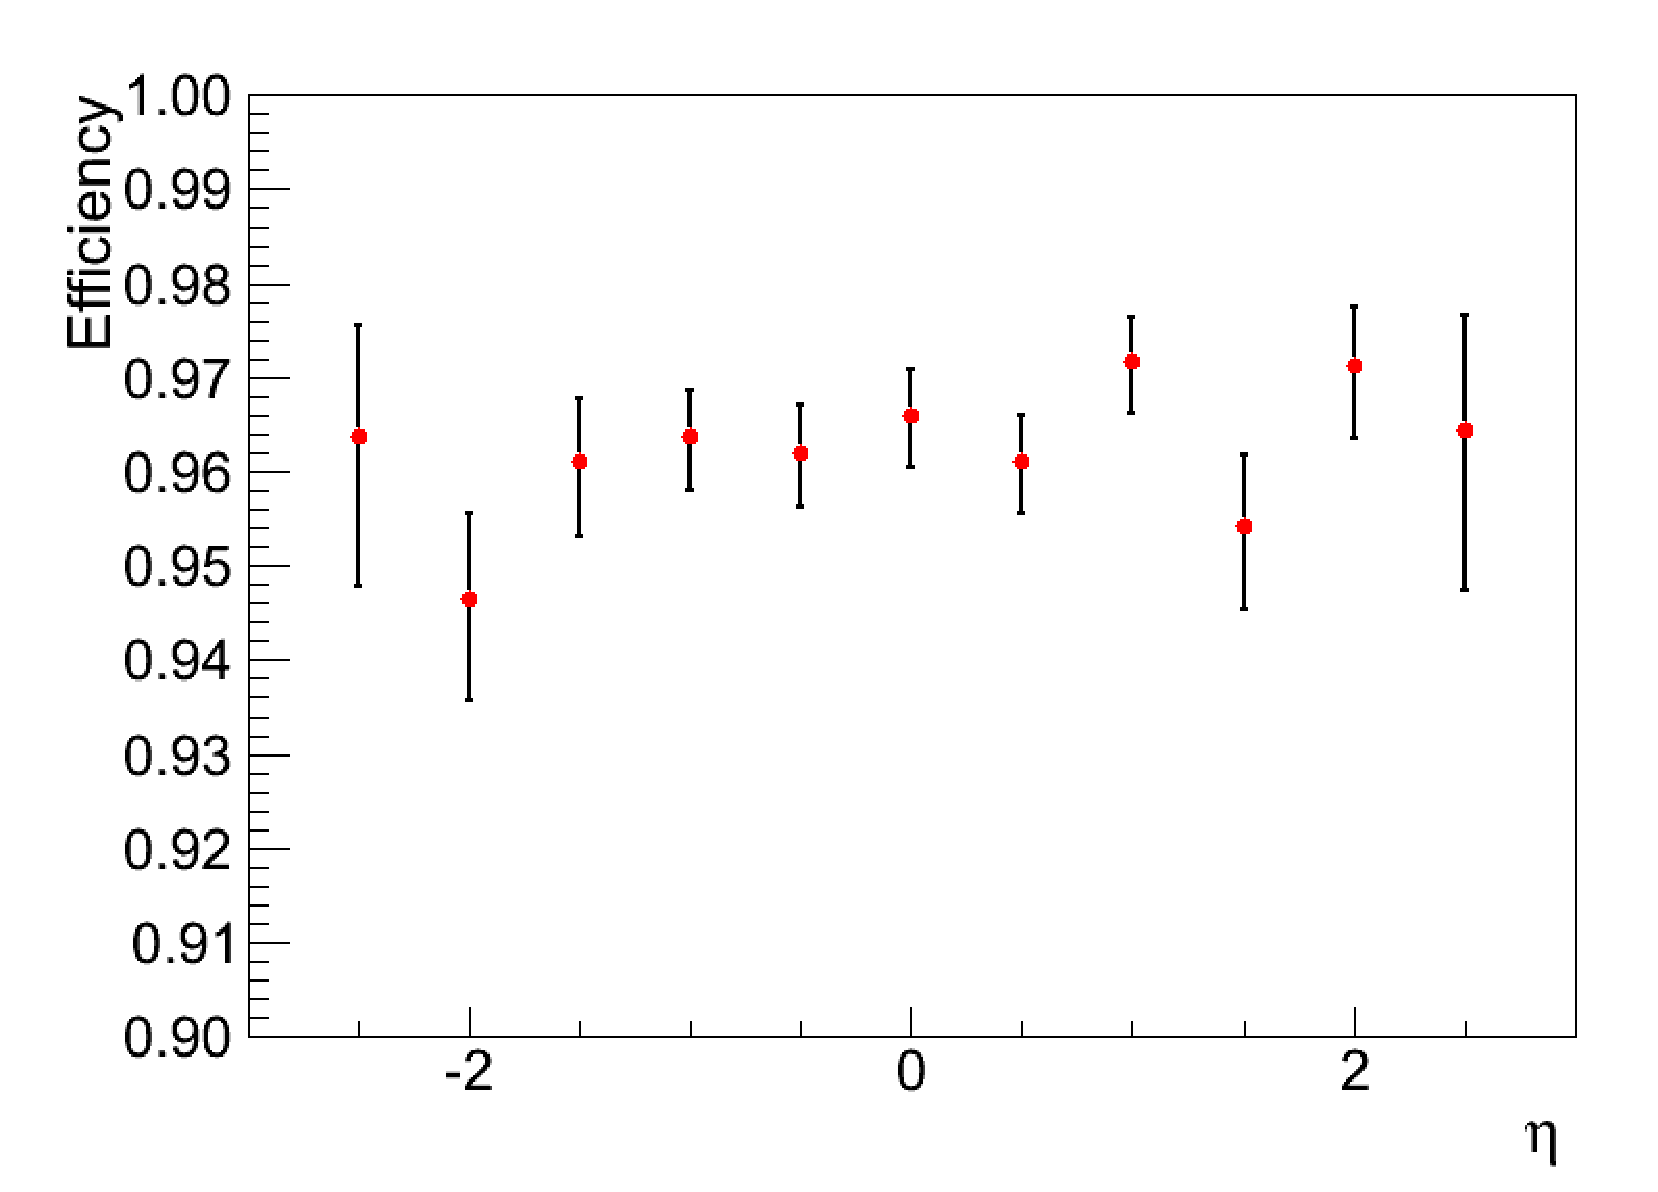
\includegraphics[width=0.48\textwidth]{figures/ElectronTriggerEffVsEta_Ele27Tight.pdf}
\end{center}
\caption{The single leg efficiency of the single electron trigger as a function of $p_{T}$ (a) and $\eta$ (b).}
\label{fig:Ele27Efficiency}
\end{figure}





%% DoubleMu7 Express : 
%% Pt10To15:
%% Barrel Eff : 25/26 = 0.961538 + 0.0318235 - 0.0828584
%% Endcap Eff : 19/20 = 0.95 + 0.0413792 - 0.105642

%% Pt15To20:
%% Barrel Eff : 81/83 = 0.975904 + 0.015537 - 0.0308607
%% Endcap Eff : 51/54 = 0.944444 + 0.0300568 - 0.051037

%% Pt20ToInf:
%% Barrel Eff : 5012/5247 = 0.955213 + 0.00285777 - 0.00303673
%% Endcap Eff : 1906/2044 = 0.932485 + 0.0055673 - 0.00600819

%% DoubleMu7 Prompt Reco : 
%% Pt10To15:
%% Barrel Eff : 33/35 = 0.942857 + 0.0367943 - 0.0703594
%% Endcap Eff : 40/43 = 0.930233 + 0.0376956 - 0.0631583

%% Pt15To20:
%% Barrel Eff : 107/108 = 0.990741 + 0.00765718 - 0.0209429
%% Endcap Eff : 82/83 = 0.987952 + 0.00996406 - 0.0271254

%% Pt20ToInf:
%% Barrel Eff : 5471/5666 = 0.965584 + 0.00242228 - 0.00259228
%% Endcap Eff : 2085/2181 = 0.955983 + 0.00439809 - 0.00483715


%% SingleMu24 Express:
%% Pt20ToInf:
%% Barrel Eff : 6345/6815 = 0.931034 + 0.00307405 - 0.00320332
%% Endcap Eff : 1412/1637 = 0.862553 + 0.00857366 - 0.00903148

%% SingleMu24 PromptReco
%% Pt20ToInf:
%% Barrel Eff : 6713/7233 = 0.928107 + 0.00304181 - 0.00316265
%% Endcap Eff : 1436/1665 = 0.862462 + 0.0085031 - 0.00895298


\subsubsection{Offline efficiency Results}

The tag definition:
\begin{itemize}
	\item  Single trigger blah
	\item Full offline electron/muon selection
\end{itemize}
	
The probe definition (muons / electrons):
\begin{itemize}
	\item  Full offline electron/muon selection
\end{itemize}

Repeat as above for each measurement, and discussions of systematics etc.


